\documentclass[12pt, a4paper]{article}
\addtolength{\oddsidemargin}{-.875in}
\addtolength{\evensidemargin}{-.875in}
\addtolength{\textwidth}{1.75in}
\addtolength{\topmargin}{-.875in}
\addtolength{\textheight}{1.75in}

\usepackage{indentfirst}
\usepackage{graphicx}
\usepackage{amsmath}


\begin{document}
\noindent
Nicholas Garrett\\ \\
Professor Dailami\\ \\
CS 3316\\ \\
11/16/2021\\ \\

\begin{center}
	\centering{	Homework Assignment 7\\ }
\end{center}


The task assigned for in this homework assignment was to build a sparse search algorithm.  The task this algorithm is expected to perform, as stated in he homework requirements, Sparse Search: Given a sorted array of strings that is interspersed with empty strings, write a method to find the location of a given string.  The assignment specified that I was to consider an algorithm capable of accomplishing this task, write a code draft of my algorithm on paper, and then write it in a programming language to verify its effectiveness.\\

When I read the algorithm prompt, I first thought of using an exhaustive search where an iterating function, such as a for loop, would iterate through the entire array of strings, comparing each key to the string being searched for.  This would have led to an algorithm of time complexity O(n), and would be fairly simple.  I kept this algorithm in the back of my mind to fall back to if I could not come up with anything else or if writing code for another algorithm proved to be too complex on paper.  \\

While I already had an idea for a simple algorithm I could use, it is the same algorithm I would assume everyone else would follow--being the easiest--and its time complexity required the algorithm to run through every single term in the array.  This is inefficient.  

In addition, though only a point I considered while writing this summary, the simple iterative search could only run on a single thread as it is forced to be a linearly calculated process; for an array of a massive size, this could slow down the calculation of the string position significantly.  So, I thought of another algorithm idea which could--in theory--run more quickly.\\

This algorithm I finally decided on is a variation on the merge sort, an algorithm I have learned extensively in my Advanced Algorithms class which seems to do the job quite well for quickly searching an array.  The reasoning I followed to choose this algorithm was twofold.  By splitting the sorted array into sub-arrays, I could only check the sections of the array where the search key could be found.  Second, by splitting the array of strings into smaller arrays, the calculation check to determine if the searched string is  comparably equivalent to the sub-string, requires only a single element to be analyzed at a time.  Additionally, as I realized later, by splitting the workload into n individual processes, these tasks are capable of being distributed among several threads and across more than a single processor--allowing for parallel programming and faster computation speeds.\\

The time I spent considering and writing this algorithm was less than I had been expecting, though I most likely was able to consider possible options more quickly due to my having recently reviewed search and sort algorithms.  From the time I started and the time I finished writing my algorithm on paper, only fifteen minutes had transpired, with most of it taken up in actually writing the code on my piece of paper.  \\

I tried to find a way to analyze the first character in each sub-string to only split it into and analyze the half which would contain the searched string.  If this had worked, the time complexity could have been decreased significantly, as only the half of the split array containing thee searched string would be checked.  Unfortunately though, I had difficulty coming up with a way to filter through the values, find the first non-empty word, and analyze the first letter of that word.  So, I unfortunately had to write a program that did not include this implementation. \\

To describe my algorithmic implementation, I made a function named "find", which took in as parameters the array, a minimum position value, a maximum position value, and the key to search for.  

First, the function calculates if there are more than a single term spanned between the minimum and maximum position values.  If there is more than 1 element in that range, then that sub-string is split in half and the function recursively calls itself with ranges of [\(min, min+\frac{max-min}{2}\)] and [\(\frac{max-min}{2}, max\)].  In other words, it splits the array in half, then each of those sub-arrays in half until it is split into n sub-arrays of a single string element. 

Then, the function checks if the sub-string is string equivalent to the searched string, and returns its position.  If one of its recursively-checked calls finds it, then it returns the position found by it.\\

In the following image, you can see the code I came up with and wrote on my scratch paper.  As you can see, I ran through a few different thoughts in how to get it to work and scratched-out redundant blocks.  Admittedly, there are a handful of fixes I would make to the code given more time in order to improve speed or efficiency, not to mention the number of operations required.  However, getting some of these to work would take time and experimentation, so I decided it would be best to leave them out.\\

\begin{figure}[ht!]
\centering
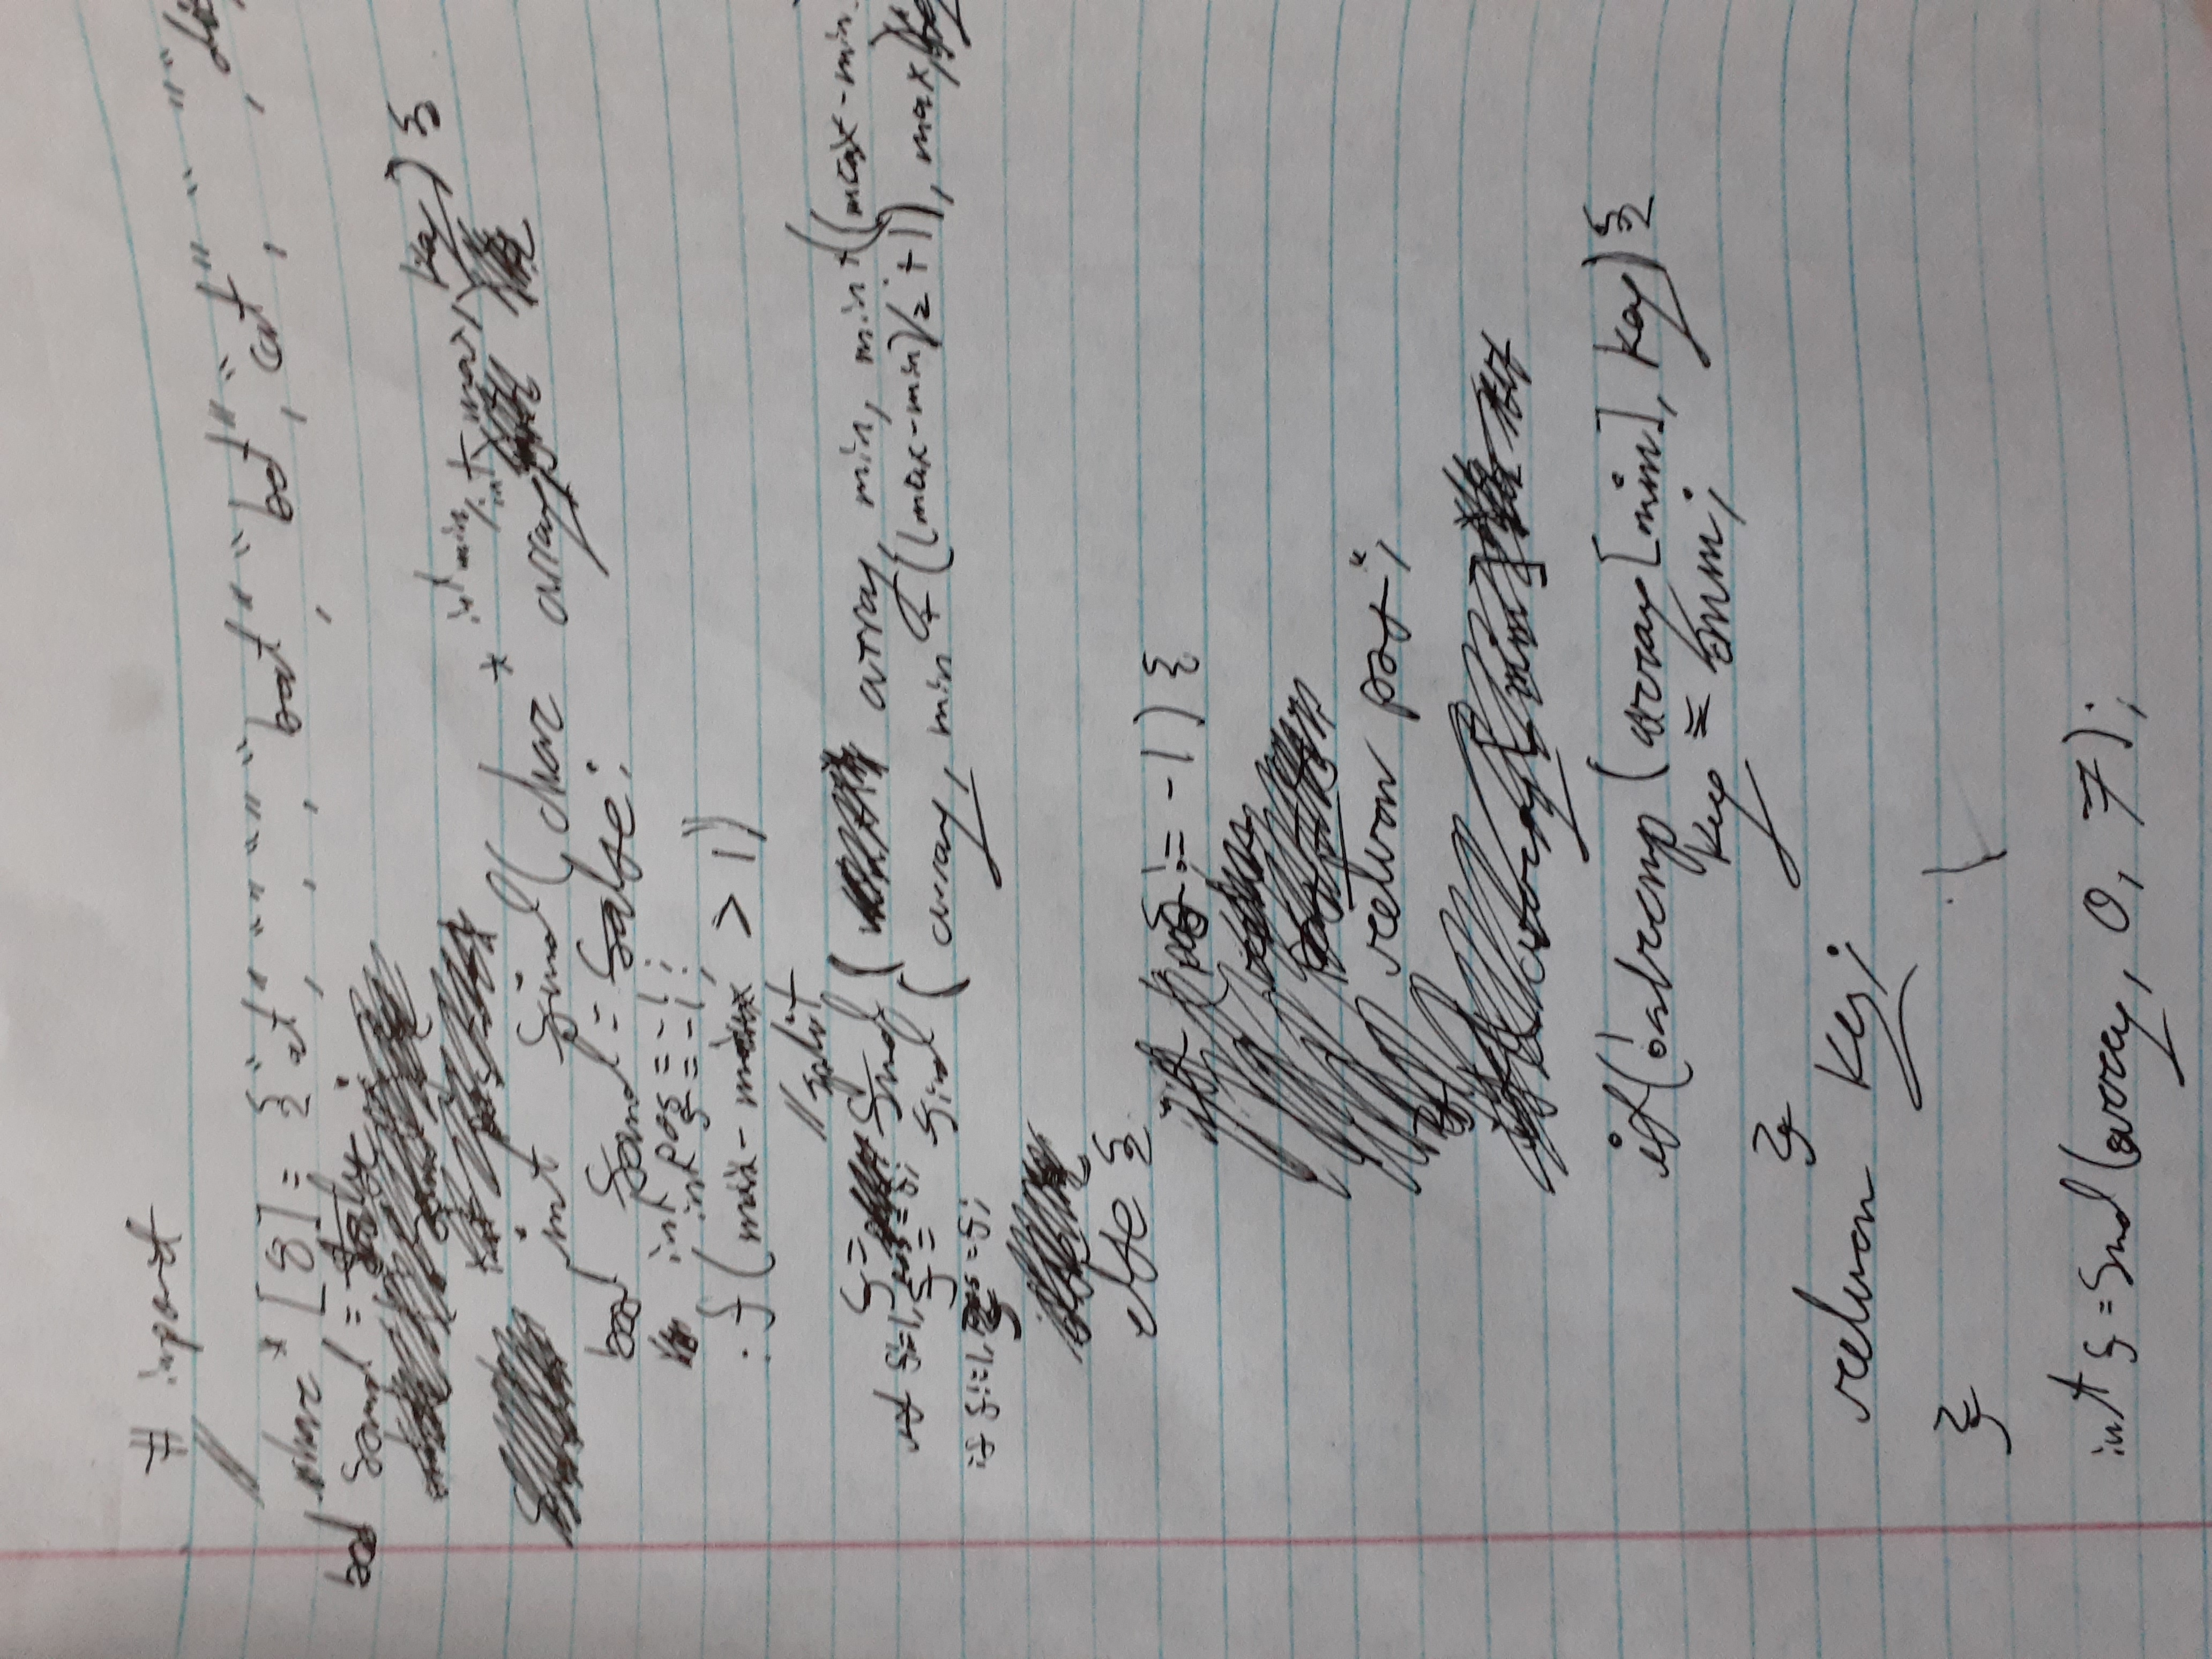
\includegraphics[width=90mm, angle=270]{paperCode}
\end{figure}

Below, I have the code I used in testing my hand-written code.\\
\begin{verbatim}
// written by Nicholas Garrett 
// 11/15/2021
/*
	Given a sorted array of strings that is interspersed with empty strings, write a method to find the location of a given string
*/ 
#include <String.h>
#include <stdio.h>
#include <stdlib.h>
#include <iostream>

using namespace std;

int find(char* array[8], int min, int max, char* key)
{
	bool found = false;
	int pos = -1;
	int f = -1;	
	
	if(abs(max-min) > 1)
	{
		f = find(array, min, min+((max-min)/2 ), key);
		if(f != -1)
		{ 
			pos = f;
		}
		

		f = find(array, min+((max-min)/2 + 1), max, key);
		if(f != -1)
		{
			pos = f;
		}
	}
	
	if(!strcmp(array[min], key))
	{
		pos = min;		
	}	
	return pos;
}

int main()
{
	char *array[7] = {"at","","","bat","cat","","deck"};
	cout << "array:";
	for(int i = 0; i < 7; i++)
	{
		cout << array[i] << ", ";	
	}
	int found = find(array, 0, 7, "cat");
	cout << "was it found? " << found;

}
\end{verbatim}

And the output for this code when searching for the string: "cat":
\begin{figure}[ht!]
\centering
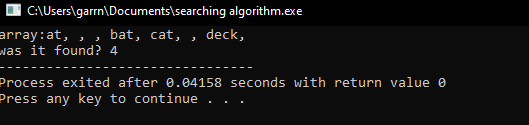
\includegraphics[width=90mm, angle=0]{codeOutput}
\end{figure} \\This is correct, as "cat" is at position 4 of the array.
\end{document}  
